\section{Galaxy model}\label{sec:galaxy-model}
The model of a galaxy used as a test bed for the implementation is a simple one.
The galaxy is assumed to comprise only two parts: a thin disk and a spherically symmetric halo.
The disk comprises a large number of particles, each representing some number of stars.
The halo is simulated as a fixed external gravitational field.
The schematic illustration of the model is shown in \autoref{fig:galaxy-model}.
\begin{figure}[htp]
    \centering
    \begin{subfigure}[t]{0.45\textwidth}
        \centering
        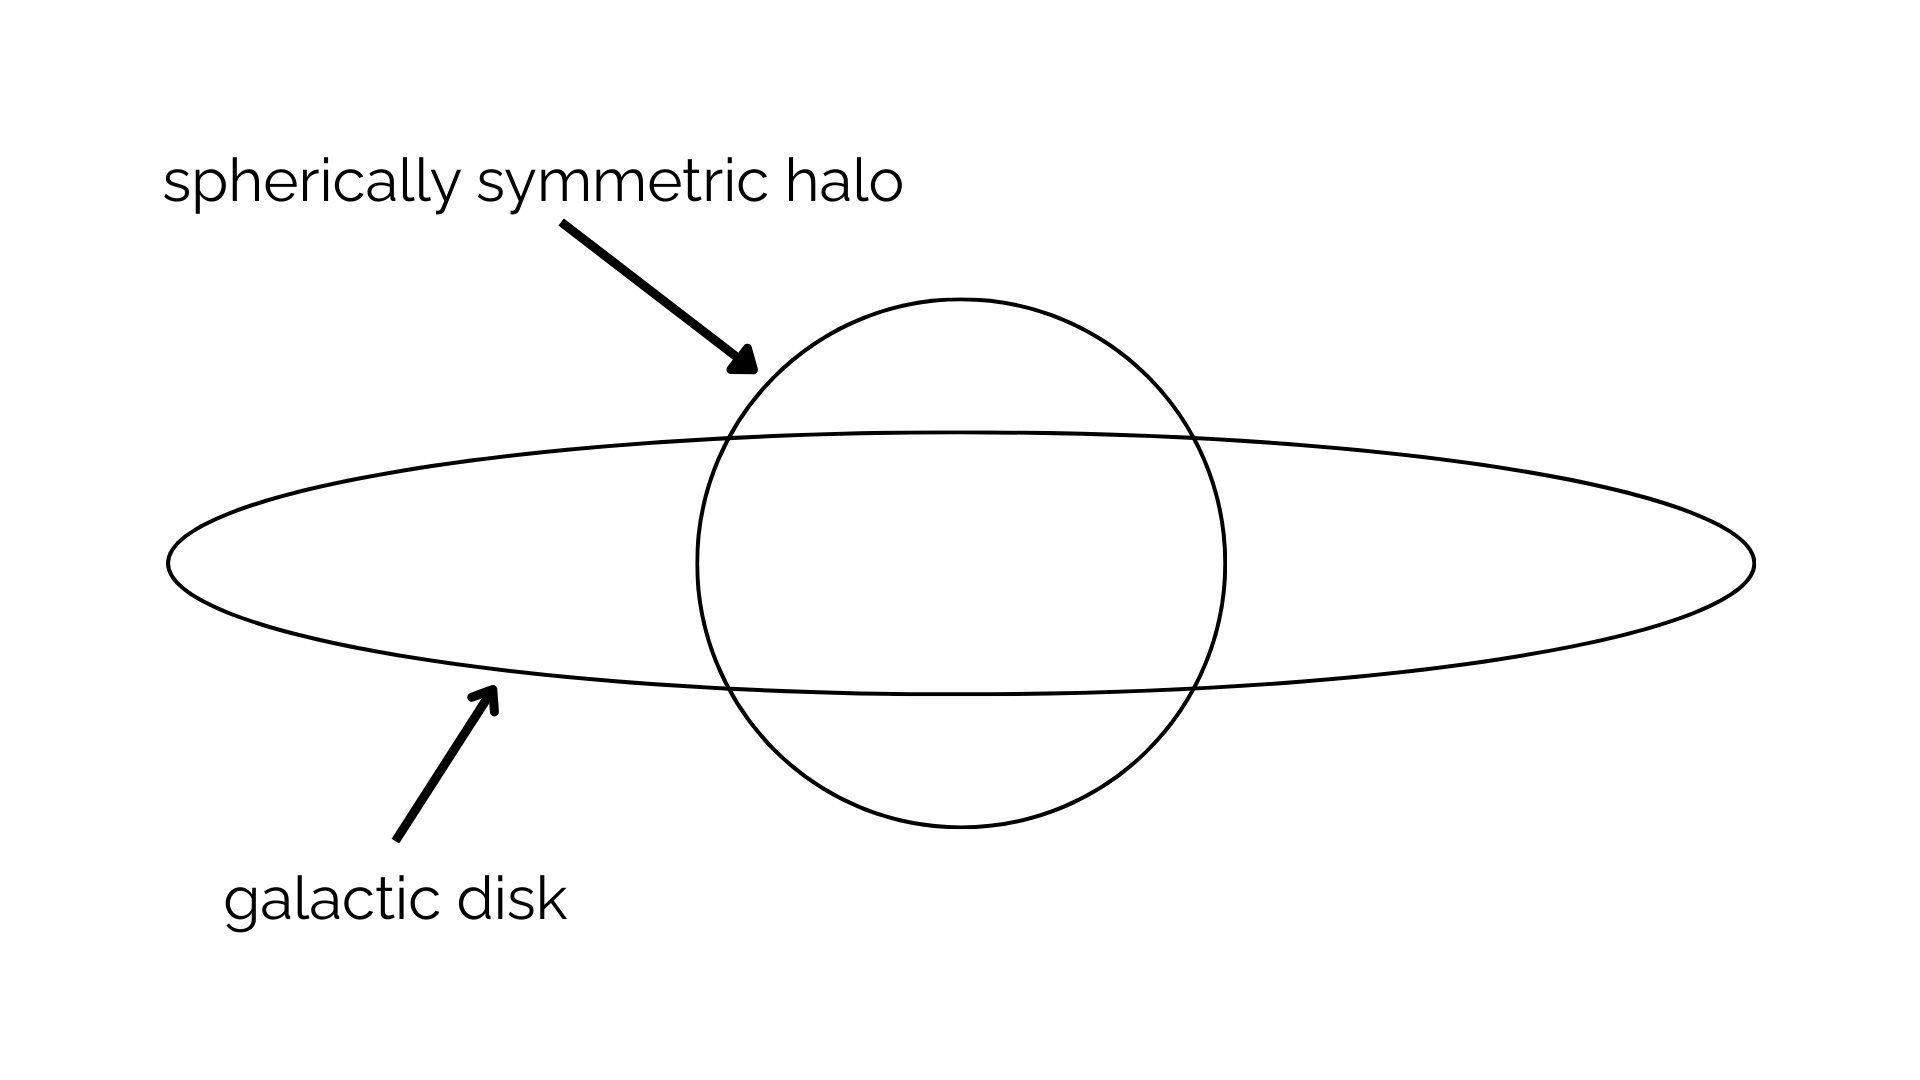
\includegraphics[scale=0.12]{img/galaxy-model.png}
        \caption{Spiral galaxy model (thin disk and spherical halo).}
        \label{fig:galaxy-model}
    \end{subfigure}
    \hfill
    \begin{subfigure}[t]{0.45\textwidth}
        \centering
        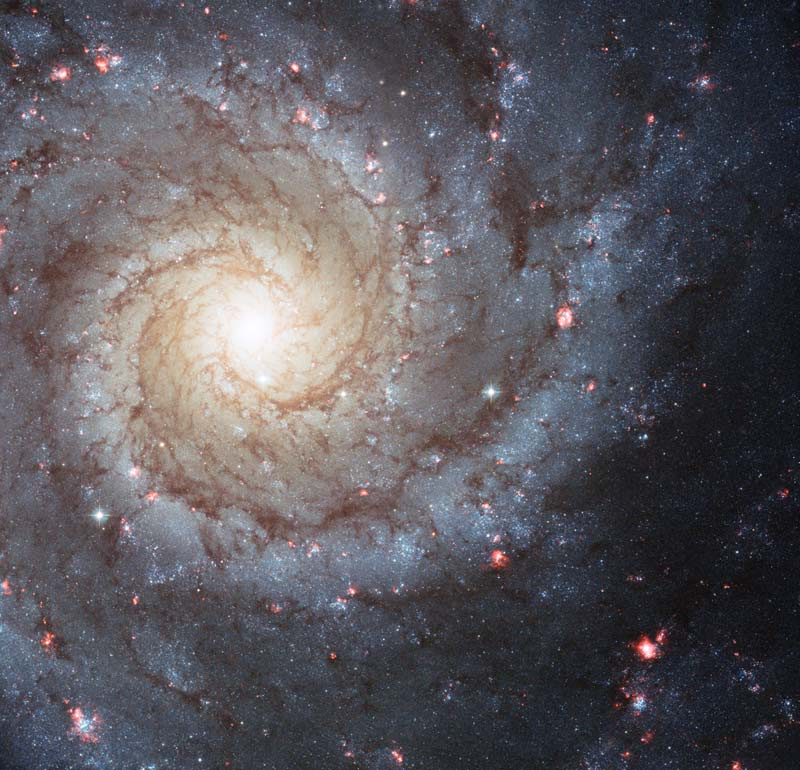
\includegraphics[scale=0.2]{img/ngc_628.jpg}
        \caption{Real-world spiral galaxy (NGC 3147).}
        \label{fig:ngc-628}
    \end{subfigure}

    \vspace{0.5em}
    {\footnotesize
        Credit for Figure~\ref{fig:ngc-628}: NASA, ESA, and the Hubble Heritage (STScI/AURA)-ESA/Hubble Collaboration;
        Acknowledgment: R. Chandar (University of Toledo) and J. Miller (University of Michigan). \par}

    \caption{Comparison between a modeled and a real-world spiral galaxy.}
    \label{fig:galaxy-comparison}
\end{figure}
\autoref{fig:ngc-628} shows an example of a real-world spiral galaxy, whose general structure we aim to reproduce.

\subsection{Disk}\label{subsec:disk}
The disk particles are sampled from a radial distribution
\begin{equation*}
    p(r) = \frac{3}{\pi R_D^2}\left(1 - \frac{r}{R_D}\right), \; z = 0,
\end{equation*}
where $R_D$ is the radius of the disk and $r \leq R_D$.
The cumulative distribution function is therefore
\begin{equation*}
    F(r, \phi) = \int_{0}^{\phi}\int_{0}^{r} p(r') r'dr'd\phi' = \frac{\phi}{2\pi R_D^3}(3R_D r^2-2r^3)
\end{equation*}
and the marginal CDFs are
\begin{equation*}
    F_R(r) = F(r, 2\pi) = \frac{1}{R_D^3}(3R_D r^2-2r^3) \quad \text{and} \quad F_\Phi(\phi) = F(R_D, \phi) = \frac{\phi}{2\pi}.
\end{equation*}
Now we use inverse transform sampling to generate initial positions $(r, \phi)$ for the particles, i.e. $\phi = 2\pi u$ and $r$ is given implicitly by $h(r) \equiv 2r^3 - 3R_D r^2 + uR_D^3 = 0$ with $u \sim U(0, 1)$.
A straightforward calculation shows that $dh/dr < 0$ for $0 < r < R_D$ and $h(0)h(R_D) < 0$ implying that $h$ has exactly one zero between 0 and $R_D$ (which can be found for example using Newton's method).

Strength of the gravitational field $\mathbf{g}_D$ due to the disk at point $\mathbf{x}_0$ lying in the disk is
\begin{equation*}
    \mathbf{g}_D = G \int_{0}^{2\pi}\int_{0}^{R_D} \sigma(r) \frac{\mathbf{x} - \mathbf{x}_0}{|\mathbf{x} - \mathbf{x}_0|^3}r dr d\phi,
\end{equation*}
where $\sigma(r) = \sigma_0(1 - r/R_D)$ describes the density profile of the disk for $r \leq R_D$.
If $M_D$ is the total mass of the disk, then $\sigma_0 = 3M_D / (\pi R_D^2)$.
By symmetry, the point $\mathbf{x}_0$ may be chosen to lie on the $x$-axis, i.e. $\mathbf{x}_0 = (-x_0, 0)$, so that $\mathbf{x} - \mathbf{x}_0 = (x_0 + r\cos\phi, r\sin\phi)$.
Letting $\bar{r} = r/R_D$ and $\bar{x}_0 = x_0 / R_D$, the integral becomes
\begin{equation*}
    \mathbf{g}_D = G\sigma_0 \int_{0}^{2\pi} \int_{0}^{1} (1 - \bar{r}) \frac{(\bar{x}_0 + \bar{r}\cos\phi, \bar{r}\sin\phi)}{|(\bar{x}_0 + \bar{r}\cos\phi, \bar{r}\sin\phi)|^3}\bar{r} d\bar{r} d\phi.
\end{equation*}
By symmetry $g_{D,y} = 0$ and thus the radial component of the field $\mathbf{g}_D$ at distance $R\bar{x}_0$ from the center is
\begin{equation}\label{eq:gx-disk}
    g_{D,r} = -|\mathbf{g}_D| = -G\sigma_0 \int_{0}^{2\pi} \int_{0}^{1} (1 - \bar{r})\frac{\bar{x}_0 + \bar{r}\cos\phi}{(\bar{x}_0^2+\bar{r}^2+2\bar{x}_0\bar{r}\cos\phi)^{3/2}}\bar{r}d\bar{r}d\phi.
\end{equation}
If the disk had constant density, $\mathbf{g}_D$ could be expressed in terms of elliptic integrals \cite{Weiss2018}.
However, to the best of the author's knowledge, the integral in \autoref{eq:gx-disk} cannot be further simplified.
For this reason, a crude approximation with a quadratic function is used: $g_{D,r} \approx a(r - h)^2 + k$, where the values $k=2.5$ and $h=0.66$ (the maximum of $g_{D,r}$ and the argument thereof) were estimated based on the graph of $g_{D,r}$ (see \autoref{fig:radial-strength-disk}).
The value of $a = -k/h^2$ can be found by setting $g_{D,r}(0) = 0$ in the approximate formula.
\begin{figure}[htp]
    \centering
    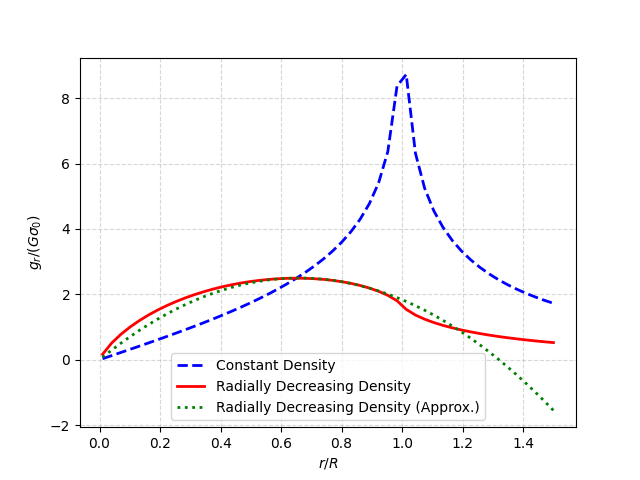
\includegraphics[scale=0.6]{img/disk-field.png}
    \caption{Magnitude of the radial component of the field strength due to a disk.
        The peak at $r=R$ for the constant density disk is in fact infinite.}
    \label{fig:radial-strength-disk}
\end{figure}

\subsection{Halo}
The density profile of the halo is analogous to the one used for the disk, save for the fact it is 3-dimensional, i.e.
\begin{equation*}
    \rho(r) =
    \begin{cases}
        \rho_0\left(1 - \frac{r}{R_H}\right), & r \leq R_H        \\
        0,                                    & \text{otherwise},
    \end{cases}
\end{equation*}
where $R_H$ is the radius of the halo.
If we let $M_H$ be the mass of the halo, then $\rho_0 = 3M_H / (\pi R_H^3)$.
Application of Gauss's law shows that we have
\begin{equation*}
    g_{H,r} = -G M_H \times
    \begin{cases}
        \frac{r}{R_H^3}\left(4 - \frac{3r}{R_H}\right), & r \leq R_H        \\
        \frac{1}{r^2},                                  & \text{otherwise}.
    \end{cases}
\end{equation*}

\subsection{Initial conditions}
The total field $\mathbf{g} = \mathbf{g}_D + \mathbf{g}_H$ is used to find initial velocities for the particles with initial positions $(x, y, 0)$.
The formula for the centripetal force yields
\begin{equation*}
    \frac{v^2}{r} = -g_r
\end{equation*}
and thus
\begin{equation*}
    \mathbf{v} = \left(-v \frac{y}{r}, v\frac{x}{r}, 0\right)
\end{equation*}
with $v = \sqrt{- r g_r}$
for counter-clockwise rotation.

\subsection{Disk with a hole}\label{subsec:disk-with-hole}
While testing the implemented methods, we observed that for modeling systems comprising multiple galaxies it may be beneficial to replace the fixed halo with a single massive particle.
In such case, the simulation turns out to stable if there are no particles in close vicinity to the galaxy center.
This means that the galactic disk ought to have a hole of radius $r_0$.
Using an approach analogous to the one used in \autoref{subsec:disk}, we obtain the following relations that can be used for sampling points $(\phi, r)$ in polar coordinates
\begin{equation*}
    \phi = 2\pi u \quad \text{ and } \quad 2(r^3 - r_0^3)-3R_D(r^2 - r_0^2) + (R_D-r_0)^2(2r_0 + R_D)u = 0,
\end{equation*}
where $u \sim U(0, 1)$.

Getting rid of the external halo field simplifies the treatment of complex systems significantly, as we do not need to keep track of the movement of the halo.
The massive particle in the galaxy center, which effectively replaces it, can be treated just as any other particle in the simulation.